\hypertarget{introduction}{%
\section{Introduction}\label{introduction}}

War pays and the line between military victories and profit blurs where
business and military networks overlap. It is no secret that profiteers
of war rarely pay for their cime. Financial crime often encourages war
itself, or rather, as one lawyer in the Democratic Republic of Congo
observed, `the lack of prosecution in the area of financial crime
encourages war crimes and war itself.'

Individuals and companies are rarely convicted for the part they play in
war, though there is precedence. In the 1948 Nuremburg Trials,
executives from the German chemical company, IG Farben, were indicted on
five counts and executed for their use role in the production of Zyklon
B.

I.G. Farben was sadly a rare case. Most businessmen, like Ernst-Wolfgan,
were never tried. He maintained to his death that the ovens they had
produced at Topf and Sons for Auschwitz, Dachau, and Buchenwald had been
misused by the Nazis. Only his brother's business partner, Kurt Prufer
was ever sentenced. The Soviets sentenced Prufer to 25 years and he died
in prison

\begin{figure}
\centering
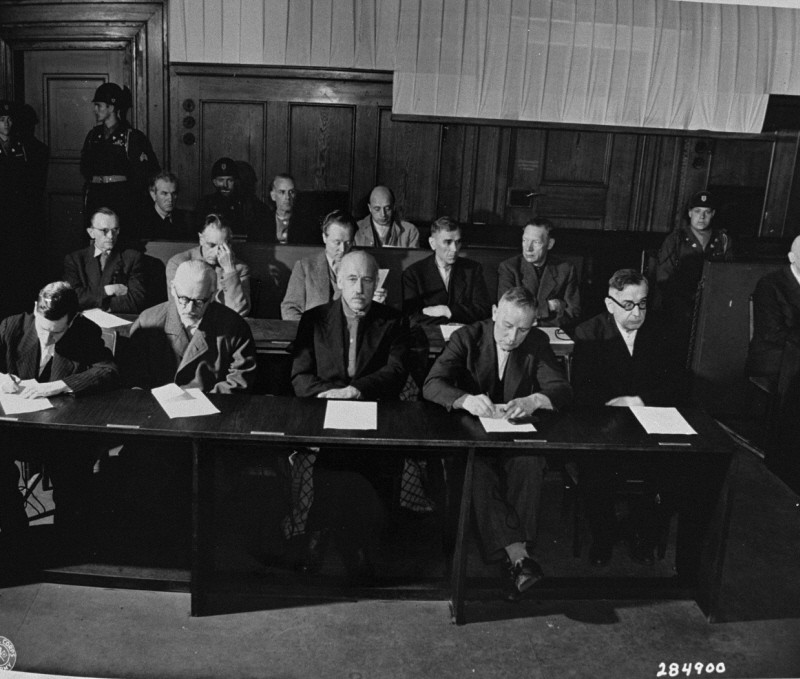
\includegraphics{../assets/IG_FARBEN.jpg}
\caption{Farben}
\end{figure}

The issue of illicit financial flows and war crimes have only become
more important since Russian actors began extracting resources from
Ukraine.

Much of the focus on illicit financial flows often falls on the
``dirty'' side of dirty money. It is known to the public that
kleptocrats and oligarchs use offshore tax havens and shell companies to
hide wealth. Less known are the reasons why London remains the dirty
money capital of the world or why Delaware is the largest secrecy
jurisdiction in the world.

Though debates surrounding privacy and public beneficial ownership
registries are public, they are not public knoweldge. In the same way
that policy debates are overlooked, so too is the role of the state in
facilitating illicit financial flows, which remains overlooked compared
to the study of how illicit financial flows against the backdrop of
corruption harm global development.

While working on the screening platforms that compliance officers use to
uphold sanctions and screen for risks, I became interested in how
effective sanctions and AML practices are in preventing state actors
from using illicit financial flows as a foreign policy tool. As part of
my research, and in light of Russia's resource grab in Ukraine, I joined
\href{https://www.osintforukraine.com/}{OSINT for Ukraine} as an
investigator. My focus is on documenting war crimes and Russia's use of
illicit funds.
